\documentclass{article}
\usepackage[utf8]{inputenc}
\usepackage{geometry}
\usepackage[T1]{fontenc}
\usepackage{amsfonts}
\usepackage{amsmath}
\usepackage{graphicx}
\usepackage{float}
\usepackage{hyperref}
\usepackage[sorting=none]{biblatex}
\usepackage{fancyhdr}
\usepackage{multicol}
\usepackage{enumitem}
\addbibresource{ref.bib}
\setlength{\columnsep}{40pt}
\setlength{\voffset}{0.7cm}
\setlength{\headsep}{40pt}
\geometry{legalpaper, portrait, margin=2cm}


% Title page
\title{Essay title\\\Large{Machine Learning, Advanced Course/DD2434/mladv24}}
\author{Aurhor \\ KTH Royal Institute of Technology\\ School of Engineering Sciences in Chemistry, Biotechnology and Health}
\date{\today}

% Header and footer
\pagestyle{fancy}
\fancyhead{}
\fancyhead[L]{\textbf{Machine Learning, Advanced Course}\\\textbf{DD2434}}
\fancyhead[R]{\textbf{Andrea Stanziale, Leonardo Lüder}\\ stanz@kth.se, luder@kth.se}
\fancyfoot{}
\begin{document}

\maketitle

% Begin page numbers
\fancyfoot[C]{\thepage}
\pagenumbering{arabic}
\begin{multicols}{2}

    \section*{1.1}
    The answers to the questions are as follows:
    \begin{itemize}[noitemsep, topsep=0pt]
        \item Yes.
        \item No.
        \item Yes.
        \item Yes
        \item No.
        \item Yes.
    \end{itemize}
    \section*{1.2}

    \subsection*{1.2.7}
    We implement a function that generates a dataset of $N$ points in the plane, where each point is drawn from a normal distribution with mean $\mu$ and precision $\tau$. For reproducability we set the seed of the random number generator to 0. We generate datasets for $N = 10, 100, 1000$ and plot the generated values as histograms, which results in figure \autoref{fig:histograms_datasets}. 

    
    \begin{figure}[H]
        \centering
        \begin{minipage}{0.49\textwidth}
            \centering
            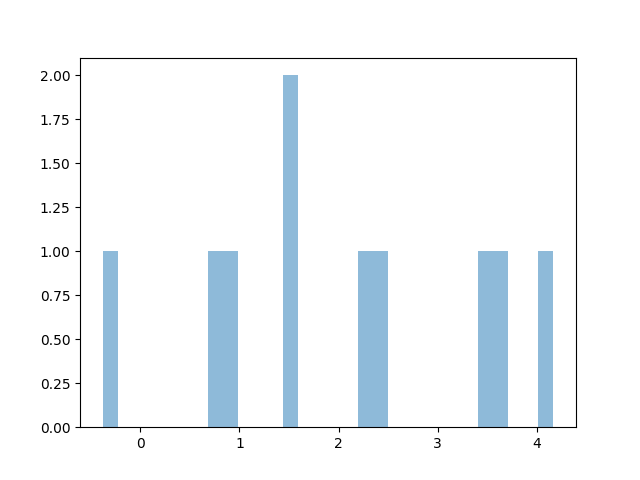
\includegraphics[width=\textwidth]{figures/1.2/dataset_1.png}
            \caption{N=10}
        \end{minipage}
        \hfill
        \begin{minipage}{0.49\textwidth}
            \centering
            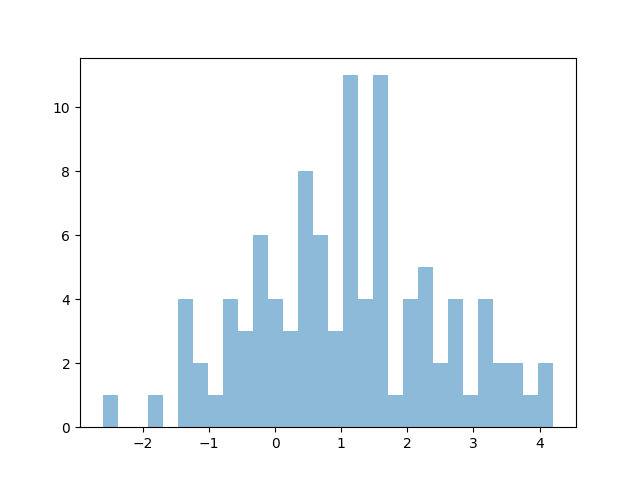
\includegraphics[width=\textwidth]{figures/1.2/dataset_2.png}
            \caption{N=100}
        \end{minipage}
        \hfill
        \begin{minipage}{0.49\textwidth}
            \centering
            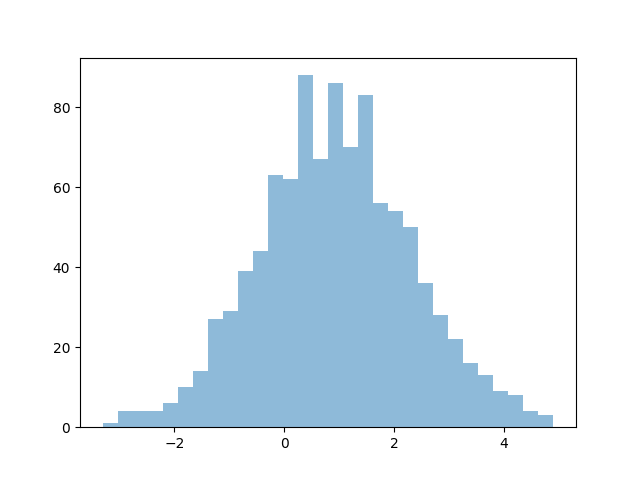
\includegraphics[width=\textwidth]{figures/1.2/dataset_3.png}
            \caption{N=1000}
        \end{minipage}
        \caption{Histograms of generated datasets}\label{fig:histograms_datasets}
    \end{figure}

    We see that the more datapoints we have the more the histogram resembles a normal distribution which is as expected.

    \subsection*{1.2.8}
    We compute the ML estimates as follows:
    \begin{align*}
        \mu_{ML} = \frac{1}{N} \sum_{i=1}^{N} X_i\\
        \tau_{ML} = \frac{N}{\sum_{i=1}^{N} {(X_i - \mu_{ML})}^2}.
    \end{align*}

    We get our results for the different datasets, with random seed $0$ as shown in table \autoref{tab:ml_estimates}.
    \begin{table}[H]
        \centering
        \begin{tabular}{|c|c|c|}     \hline
            N & $\mu_{ML}$ & $\tau_{ML}$ \\
            \hline
            10      &   2.043   &   0.535\\
            100     &   1.085   &   0.492\\
            1000    &   0.936   &   0.513\\
            \hline
        \end{tabular}
        \caption{ML estimates for different datasets}
        \label{tab:ml_estimates}
    \end{table}
    We see, that the higher the number of datapoints, the closer the ML estimates are to the true values of $\mu = 1$ and $\tau = 0.5$.


    \subsection*{1.2.9}

    We derive an expression for the exact posterior. We have the likelihood function $p(X|\mu, \tau)$ and the prior distributions $p(\mu|\tau)$ and $p(\tau)$. We can write the joint posterior as:

    \begin{equation}
        p(\mu, \tau | X) \propto p(X | \mu, \tau) p(\mu | \tau) p(\tau)
    \end{equation}


    The likelihood is given by:

    \begin{equation}
    p(X | \mu, \tau) = \prod_{i=1}^{N} p(X_i | \mu, \tau) = \prod_{i=1}^{N} \sqrt{\frac{\tau}{2 \pi}} e^{-\frac{\tau}{2} (X_i - \mu)^2}
    \end{equation}

    where we assume \( X_i | \mu, \tau \sim N(\mu, \frac{1}{\tau}) \).

    The prior distributions are:

    \begin{equation}
    p(\mu | \tau) = N(\mu_0, \frac{1}{\lambda_0 \tau}); \quad p(\tau) = \mathrm{Gamma}(\alpha_0, \beta_0)
    \end{equation}


    This gives the joint posterior:

    \begin{multline}
    p(\mu, \tau | X) \propto \prod_{i=1}^{N} \sqrt{\frac{\tau}{2 \pi}} e^{-\frac{\tau}{2} (X_i - \mu)^2} \times \sqrt{\frac{\lambda_0 \tau}{2 \pi}} e^{-\frac{\lambda_0 \tau}{2} (\mu - \mu_0)^2}\\ \times \frac{\beta_0^{\alpha_0}}{\Gamma(\alpha_0)} \tau^{\alpha_0 - 1} e^{-\beta_0 \tau}
    \end{multline}

    Simplifying, we get:

    \begin{equation}
    p(\mu, \tau | X) \propto \left(\frac{\tau}{2 \pi}\right)^{\frac{N+1}{2}} e^{-\frac{\tau}{2} \left(\sum_{i=1}^{N} (X_i - \mu)^2 + \lambda_0 (\mu - \mu_0)^2 + 2 \beta_0 \right)} \tau^{\alpha_0 + \frac{N}{2} - 1}
    \end{equation}


    After completing the square for terms involving \( \mu \) and simplifying, the posterior distribution of \( \mu \) given \( X \) and \( \tau \) is:

    \begin{equation}
    p(\mu | X, \tau) \sim N\left(\frac{\sum X_i + \lambda_0 \mu_0}{N + \lambda_0}, \frac{1}{(N + \lambda_0) \tau}\right).
    \end{equation}

    The implementation in Code is given under 1.2.9 in the appended Jupiter Notebook.

    \subsection*{1.2.10}

    We implement the CAVI algorithm for the system described in Bishop 10.24. We introduce the prior parameters as:
    \begin{equation*}
        \mu_0 = 0; \,
        \lambda_0 = 0.1;\,
        a_0 = 0.1;\,
        b_0 = 0.1
    \end{equation*}
    We choose these values for the prior parametes, as we want a more data driven approach for the sake of this exercise. A small value for the prior precision $\lambda_0$ and the shape parameter $a_0$ will make the prior less informative. $\mu_0$ is set to zero, as our guess for the mean and we set $b_0$ to a small value to indicate a broader prior.

    \par
    We run the CAVI algorithm with a tolerance of $10^{-12}$ and plot the ELBO at each iteration for every dataset. The results are shown in figure \autoref{fig:elbo}. We see that the ELBO converges to a local maximum for all datasets while being monotonically increasing.

    \begin{figure}[H]
        \centering
        \begin{minipage}{0.49\textwidth}
            \centering
            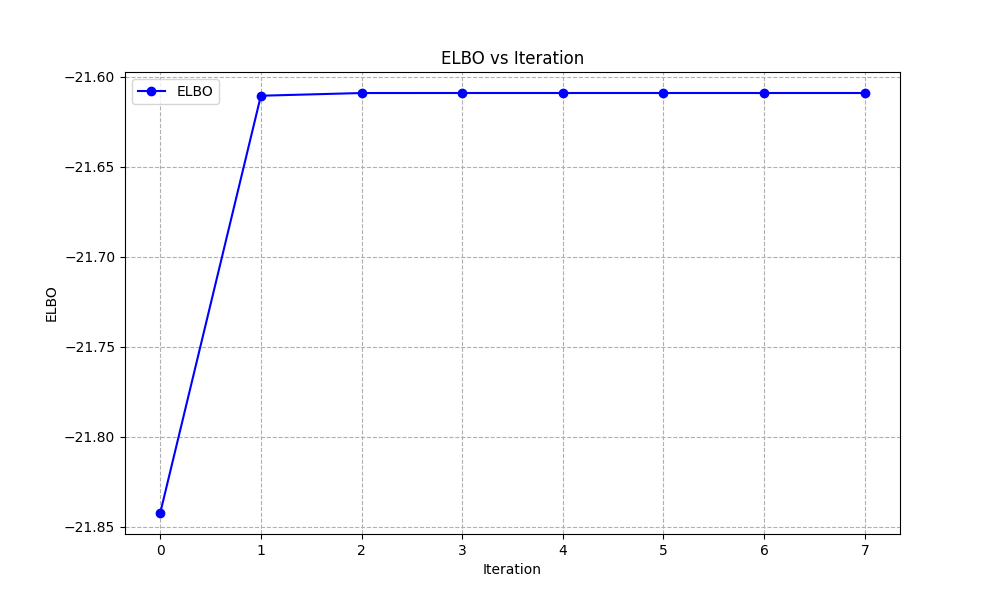
\includegraphics[width=\textwidth]{figures/1.2/elbos_d1.png}
            \caption{N=10}
        \end{minipage}
        \hfill
        \begin{minipage}{0.49\textwidth}
            \centering
            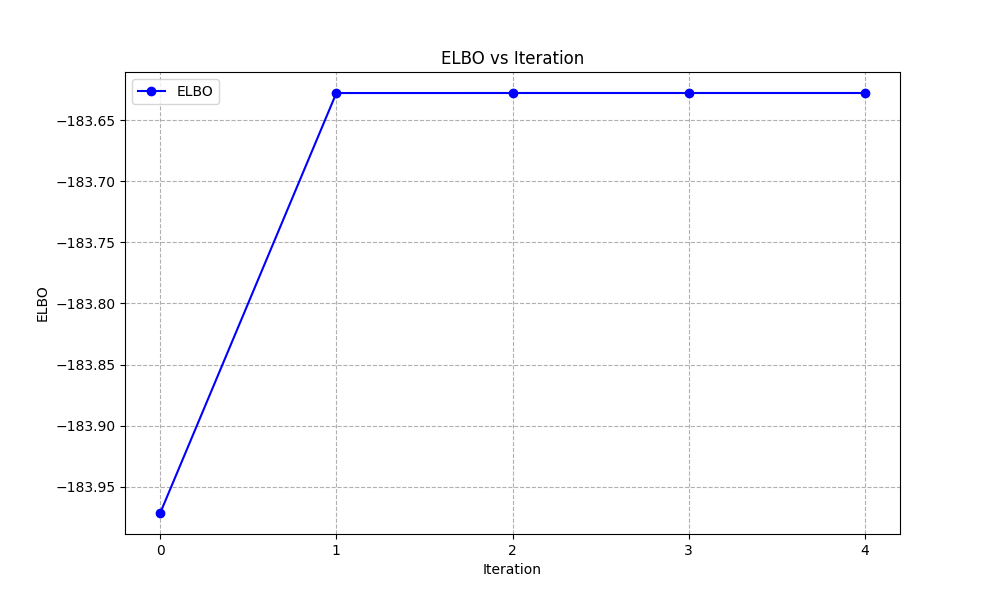
\includegraphics[width=\textwidth]{figures/1.2/elbos_d2.png}
            \caption{N=100}
        \end{minipage}
        \hfill
        \begin{minipage}{0.49\textwidth}
            \centering
            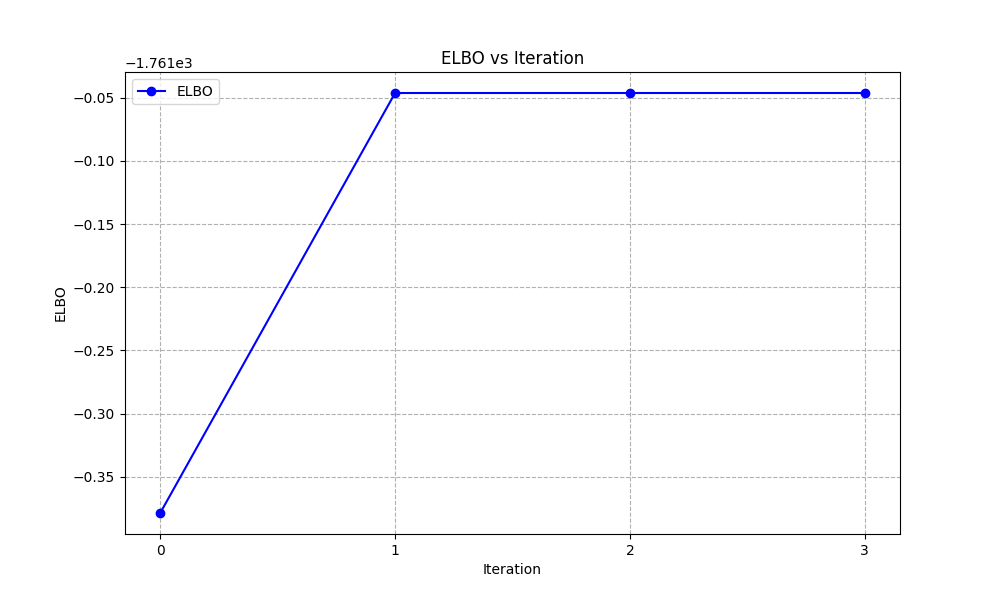
\includegraphics[width=\textwidth]{figures/1.2/elbos_d3.png}
            \caption{N=1000}
        \end{minipage}
        \caption{ELBO for different datasets}\label{fig:elbo}
    \end{figure}

    We also plot the posterior mean and variance for $\mu$ and $\tau$ for each dataset. The results are shown in figure \autoref{fig:posterior}. 

    \begin{figure}[H]
        \centering
        \begin{minipage}{0.49\textwidth}
            \centering
            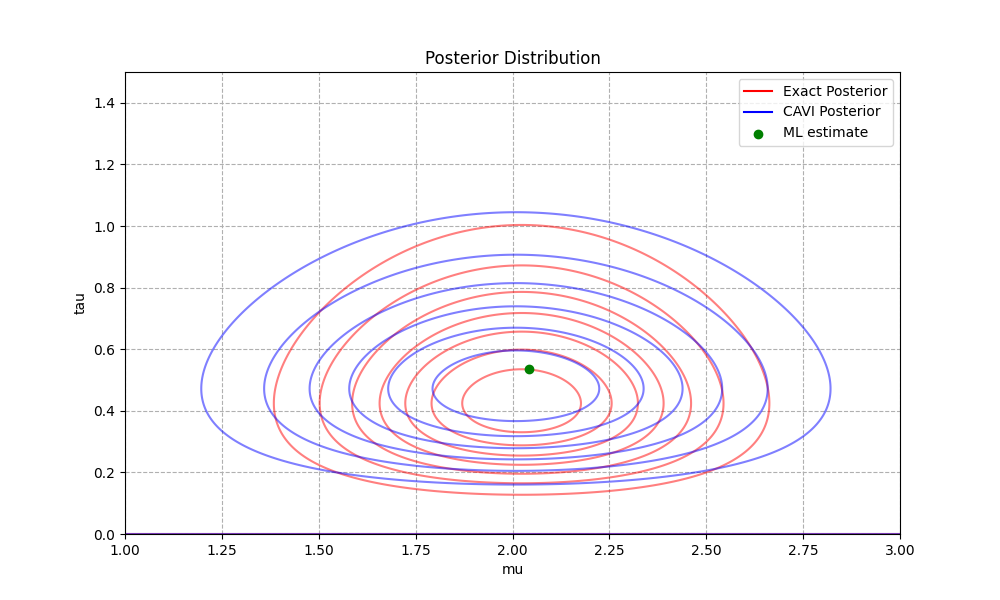
\includegraphics[width=\textwidth]{figures/1.2/contour_d1.png}
            \caption{N=10}
        \end{minipage}
        \hfill
        \begin{minipage}{0.49\textwidth}
            \centering
            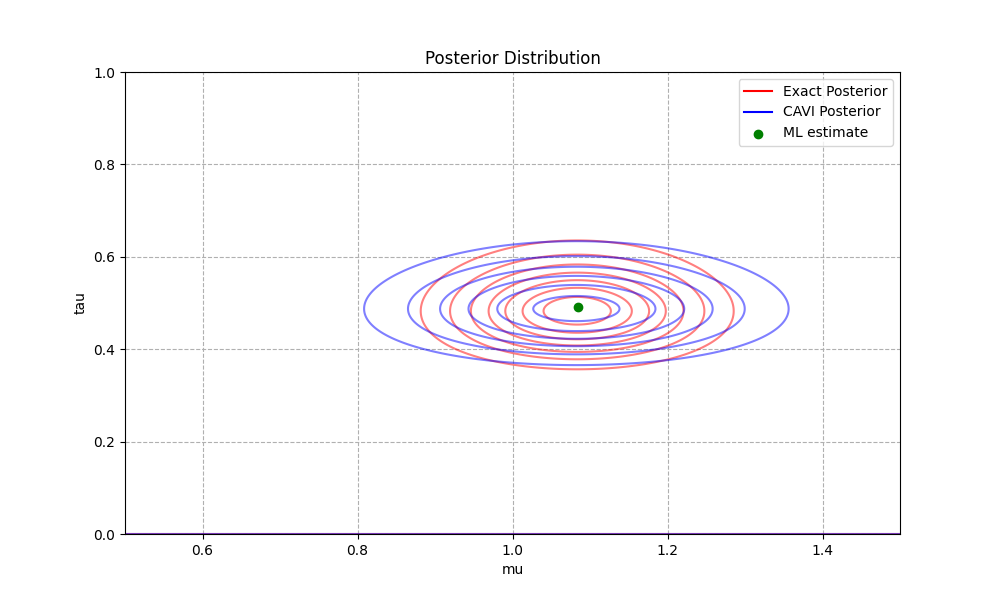
\includegraphics[width=\textwidth]{figures/1.2/contour_d2.png}
            \caption{N=100}
        \end{minipage}
        \hfill
        \begin{minipage}{0.49\textwidth}
            \centering
            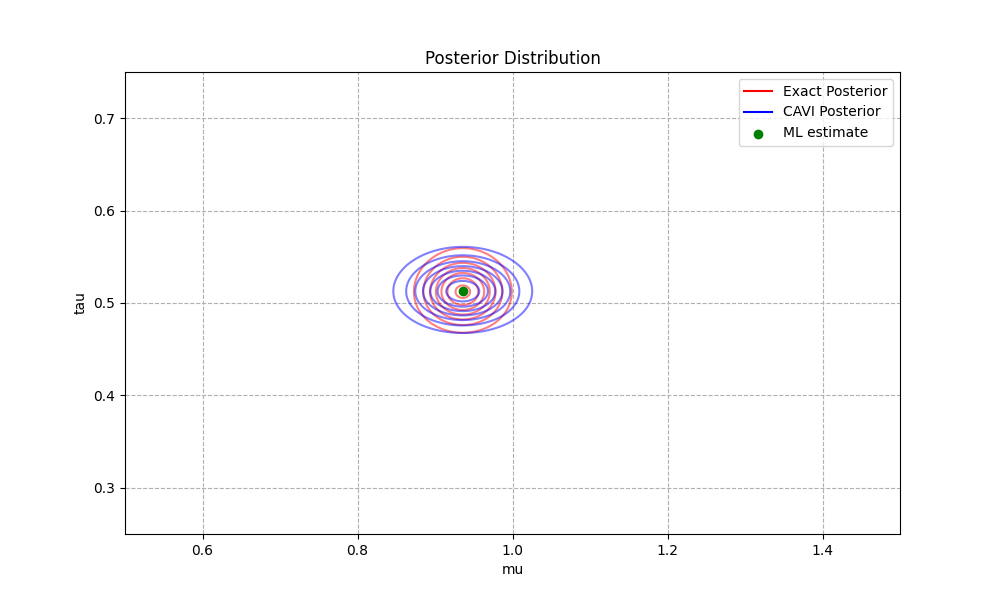
\includegraphics[width=\textwidth]{figures/1.2/contour_d3.png}
            \caption{N=1000}
        \end{minipage}
        \caption{Posterior for different datasets}\label{fig:posterior}
    \end{figure}

    We see, that the exact posterior is well approximated by the CAVI algorithm. The posterior mean and variance for $\mu$ and $\tau$ converge to the true values as the number of datapoints increases.

    

\end{multicols}
\clearpage
\addcontentsline{toc}{section}{References}
% \printbibliography{}

\end{document}
